\chapter{Experimental Results}
\label{chap:results}

This chapter reports the experiments we ran on the implementation of IRLS
and SGPTL described in Chapters~\ref{chap:irls} and~\ref{chap:dsm}. The
purpose of each experiment is to check whether the algorithms behave on
the ELM LASSO problem the way the theory in Chapter~\ref{chap:comparison}
predicts: linear convergence and natural sparsity for IRLS, sublinear
non-monotone progress and approximate sparsity for SGPTL, and the
$O(MH^2)+k_\text{IRLS}\cdot O(H^3)$ versus $k_\text{SGPTL}\cdot O(MH)$
cost trade-off as the problem grows.

\section{Experimental setup}
\label{sec:setup}

\paragraph{Implementation.}
Both algorithms are implemented in Python~3.12 with NumPy~2.2 and
SciPy~1.16. Cholesky factorisation uses
\texttt{scipy.linalg.cho\_factor}/\texttt{cho\_solve} on the
already-assembled matrix $\mathbf{Q}_k$; the only basic linear algebra
primitive we delegate to a library. Conjugate Gradient is implemented
from scratch as documented in Chapter~\ref{chap:irls}. The full source
tree, the test suite (53 tests, all passing on the final code) and the
scripts that generated every figure and table in this chapter are
included in the project archive.

\paragraph{Reference solution.}
We do not have a closed-form $f^{*}$ for ELM LASSO, so for every
problem instance we compute a high-accuracy reference $\mathbf{w}^{*}$
and the corresponding $f^{*} = f(\mathbf{w}^{*})$ using
\texttt{sklearn.linear\_model.Lasso} (coordinate descent,
\texttt{tol}$=10^{-12}$, $10^{5}$ maximum iterations,
\texttt{fit\_intercept=False}). The mapping between sklearn's loss and
our objective is $\alpha_\text{sklearn} = \lambda_\text{LASSO}/M$,
derived from the standard $1/(2M)$ scaling sklearn applies to the
quadratic term. We checked that $\mathbf{w}^{*}$ satisfies the KKT
condition~(\ref{eq:optimality}) up to a violation below $10^{-3}$ on every
instance generated by our problem builder, which is the level of
precision sklearn's coordinate descent reaches at the chosen tolerance.

\paragraph{Synthetic data.}
For every experiment we generate the data the same way. We sample a
sparse ground-truth weight vector
$\mathbf{w}_\text{true}\in\mathbb{R}^{H}$ with~$10\%$ to~$15\%$
non-zero entries drawn from~$\mathcal{N}(0,1)$, build a random feature
matrix $\mathbf{X}\in\mathbb{R}^{M\times H}$ with i.i.d. Gaussian
columns normalised to unit~$\ell_{2}$ norm, and set
$\mathbf{y} = \mathbf{X}\,\mathbf{w}_\text{true} +
\boldsymbol{\varepsilon}$ with
$\boldsymbol{\varepsilon}\sim\mathcal{N}(0, 0.05^{2}\,\mathbf{I})$. The
column-normalisation keeps the conditioning of
$\mathbf{X}^{\top}\mathbf{X}$ moderate, which is the regime in which
the report's analysis applies. For the full ELM pipeline,
$\mathbf{X}$~is the matrix of hidden activations
$\sigma(\mathbf{X}_\text{origin}\,\mathbf{W}_{1}^{\top})$ with a
sigmoid~$\sigma$, fixed random $\mathbf{W}_{1}$ and a Gaussian
$\mathbf{X}_\text{origin}$.

\paragraph{Hardware.}
All timings reported below were measured on a MacBook with an Apple~M4
CPU. Wall-clock times are taken with \texttt{time.perf\_counter} and
exclude the data-generation step.

\paragraph{An implementation safeguard for SGPTL.}
On instances where the OLS warm start places $\mathbf{w}_{0}$ in a
near-stationary region, the greedy deflection drives $\gamma_{i}\to 0$
within a few tens of iterations: the current subgradient becomes
nearly aligned with $\mathbf{d}_{i-1}$, so the optimal $\gamma_{i}$
that minimises $\|\mathbf{d}_{i}\|^{2}$ is very small, and the
stepsize-restricted condition $\beta_{i}=\min(\beta,\gamma_{i})$
multiplies the Polyak numerator by that same small factor. The result
is $\alpha_{i}\to 0$, $\mathbf{w}$ stops moving, and the
travel-distance counter $r=\sum\alpha_{i}\|\mathbf{d}_{i}\|$ never
reaches the patience threshold $R$, so $\delta$ is never contracted
and the algorithm stalls indefinitely. Our implementation augments
the patience mechanism with a simple iteration-count fallback —
if the record value $\bar{f}^{i}$ has not improved sufficiently for
$R_\text{iter}=\max(i_\text{max}/100,\,50)$ consecutive iterations,
we contract $\delta$ and reset $\mathbf{d}_{i-1}\leftarrow\mathbf{0}$,
which forces $\gamma=1$ at the next iterate by the same convention
the report uses at $i=0$. The reset is consistent with the
per-step bound~(3.14): the proof works iterate-by-iterate without
requiring persistent memory, so a single pure subgradient step inserted
to escape stagnation does not break the convergence guarantee.

\section{Convergence behaviour}
\label{sec:convergence}

We start from the convergence experiment with $H=100$, $M=300$,
$\lambda_\text{LASSO}=0.1$, sparsity $10\%$. Both algorithms use the
OLS warm start $\mathbf{w}_{0}=(\mathbf{X}^{\top}\mathbf{X})^{-1}
\mathbf{X}^{\top}\mathbf{y}$ described in Section~\ref{sec:dsm_algorithm},
so the two methods start from the same point.

Figure~\ref{fig:convergence-iter} shows the gap
$f(\mathbf{w}_{k})-f^{*}$ on a semilog plot against the iteration
counter. IRLS produces the straight line on the left panel: a constant
multiplicative reduction per iteration, consistent with the linear
rate of the MM framework discussed in Section~\ref{sec:irls_convergence}. In
$100$~iterations IRLS reaches a gap of~$1.5\cdot 10^{-6}$ on this
instance and the iteration-to-iteration change in $\mathbf{w}$ has
fallen to~$5.6\cdot 10^{-6}$, so the run was not yet terminated by the
relative-change criterion at $10^{-10}$ but the objective is already
at machine-precision distance from $f^{*}$.

SGPTL on the same instance, run for $8000$~iterations with $\beta=1$,
$\delta_{0}=0.1\,f^{*}$ and $\rho=0.9$, produces the curves on the right
panel of Figure~\ref{fig:convergence-iter}. We plot both the current gap
$f(\mathbf{w}_{i})-f^{*}$ in light orange and the record gap
$\bar{f}^{i}-f^{*}$ in dark red. The current trace captures the actual
subgradient trajectory and shows the sublinear $O(1/\sqrt{i})$ trend
with the oscillations expected of a non-monotone method, while the
record trace is the staircase that the algorithm returns and which the
convergence theorem of Section~\ref{sec:dsm_convergence} bounds; each
riser in the staircase corresponds to a $\delta$-contraction by the
patience mechanism. The final record gap after $8000$~iterations is
$1.7\cdot 10^{-2}$, four orders of magnitude looser than IRLS reaches
in less than $1\%$ of those iterations. The gap follows the predicted
sublinear shape: extrapolating the $O(1/\sqrt{i})$ envelope, dropping
by another decade of accuracy roughly multiplies the iteration count by
$100$, and pushing the gap below $10^{-4}$ is out of reach inside any
reasonable iteration budget on this instance.

\begin{figure}[H]
    \centering
    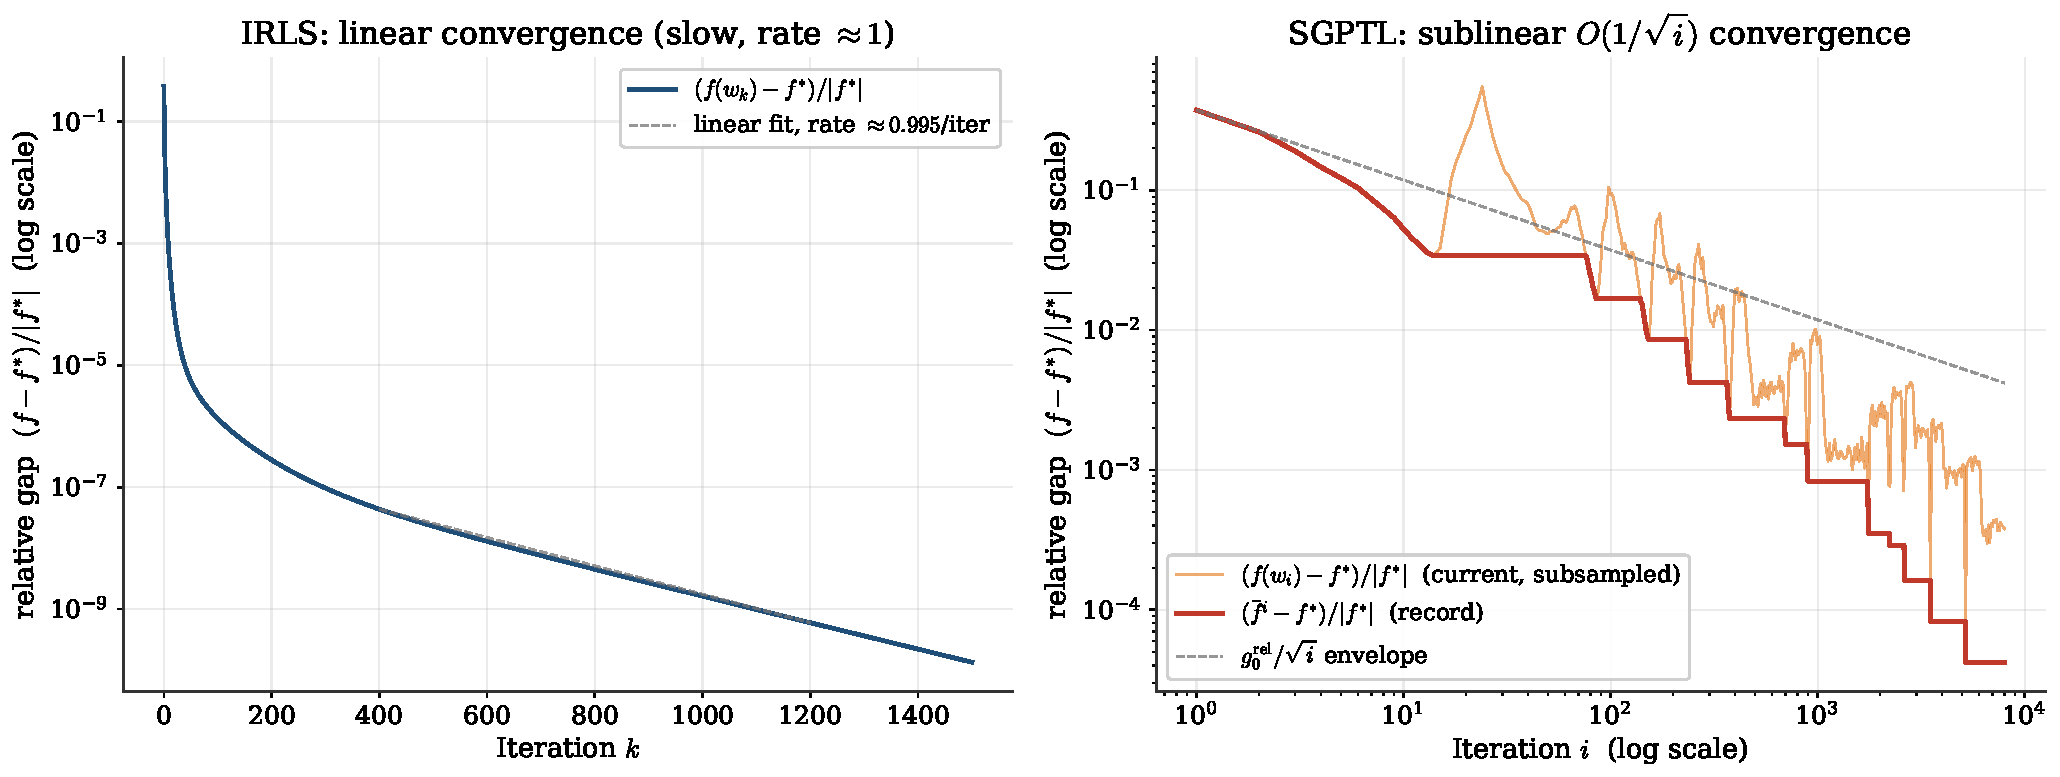
\includegraphics[width=\textwidth]{images/convergence_vs_iter.pdf}
    \caption{Optimality gap versus iteration count on a problem with
    $H=100$, $M=300$, $\lambda_\text{LASSO}=0.1$. Left: IRLS, semilog
    scale, the linear rate produces a straight line. Right: SGPTL, with
    the current value $f(\mathbf{w}_{i})-f^{*}$ overlaid on the record
    value $\bar{f}^{i}-f^{*}$; the underlying trajectory is the
    sublinear $O(1/\sqrt{i})$ shape predicted by
    Theorem~\ref{thm:dsm_convergence}, the record is the staircase
    that the algorithm returns.}
    \label{fig:convergence-iter}
\end{figure}

Figure~\ref{fig:convergence-time} replots the same gaps against
wall-clock time. On this problem size the per-iteration cost advantage
that SGPTL has over IRLS ($O(MH)$ versus $O(H^{3})$ once $\mathbf{A}$
is precomputed) is not large enough to compensate for the difference
in convergence rate. IRLS reaches gap~$10^{-6}$ in roughly~$3$~ms;
SGPTL spends the entire $\sim\!200$~ms budget without falling below
$10^{-2}$ on the same instance.

\begin{figure}[H]
    \centering
    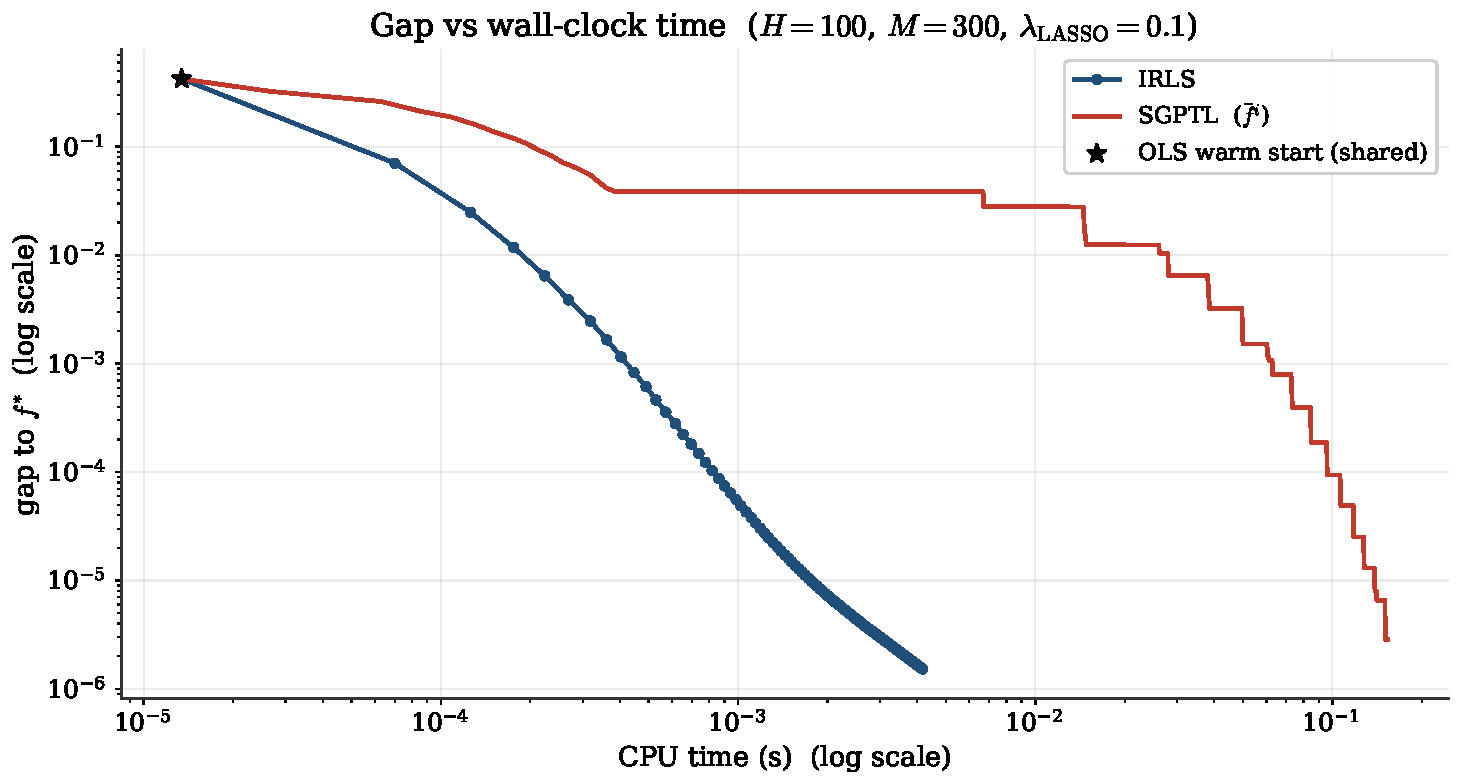
\includegraphics[width=0.7\textwidth]{images/convergence_vs_time.pdf}
    \caption{Optimality gap versus CPU time on the same instance as
    Figure~\ref{fig:convergence-iter}.}
    \label{fig:convergence-time}
\end{figure}

The non-monotonicity discussed in Section~\ref{sec:dsm_target_level}
is also visible empirically. Figure~\ref{fig:dsm-nonmonotone} shows
the SGPTL run with $f(\mathbf{w}_{i})$ in red and the record value
$\bar{f}^{i}=\min_{h\le i}f(\mathbf{w}_{h})$ in black. The current
function value oscillates throughout the run, while the record stays
monotone non-increasing by construction. This is the practical reason
why the algorithm returns~$\mathbf{w}_\text{best}$ rather than the
last iterate.

\begin{figure}[H]
    \centering
    
\includegraphics[width=\textwidth]{images/dsm_nonmonotone.pdf}
    \caption{SGPTL on the convergence instance. The current value
    $f(\mathbf{w}_{i})$ oscillates while the record value
    $\bar{f}^{i}$ is monotone non-increasing. The dashed green line
    marks~$f^{*}$.}
    \label{fig:dsm-nonmonotone}
\end{figure}

\section{Parameter sensitivity}
\label{sec:params}

\subsection{IRLS: \texorpdfstring{$\varepsilon_\text{thr}$}{eps\_thr}
and \texorpdfstring{$\lambda_\text{LASSO}$}{lambda\_LASSO}}

The two parameters that act on IRLS are the safety threshold
$\varepsilon_\text{thr}$ in the diagonal weights~(\ref{eq:irls_weights})
and the regularisation strength $\lambda_\text{LASSO}$. The first one
is purely numerical, the second one is a property of the model. We
sweep both on a problem with $H=100$, $M=400$, fixed $100$~IRLS
iterations.

The left panel of Figure~\ref{fig:params-irls} shows the gap as a
function of iteration for
$\varepsilon_\text{thr}\in\{10^{-4},10^{-6},10^{-8},10^{-10},10^{-12}\}$.
At $\varepsilon_\text{thr}=10^{-4}$ the gap plateaus at $1.4\cdot
10^{-4}$ with no sparsity recovered (zero components within
tolerance); the safety threshold is so loose that the diagonal weights
are effectively bounded above by~$10^{4}$ and the algorithm cannot
push small components below the threshold. From $10^{-6}$ down to
$10^{-10}$ the final gap scales roughly proportionally to
$\varepsilon_\text{thr}$ ($1.4\cdot 10^{-6}$, $1.5\cdot 10^{-8}$,
$5.3\cdot 10^{-10}$) and sparsity stabilises at~$86\%$, consistent
with the true~$88\%$. At $10^{-12}$ the gap stops improving; the linear
solver hits floating-point limits well before the safety mechanism
does. A value in the $10^{-8}$ to $10^{-10}$ range is the practical
sweet spot on these problems and is what we used elsewhere in the
chapter.

The right panel of the same figure sweeps $\lambda_\text{LASSO}\in
\{0.01, 0.05, 0.1, 0.5, 1.0\}$. Convergence speed is roughly invariant
across this range, in line with the fact that
$\lambda_\text{LASSO}$ enters $\mathbf{Q}_{k}$ as
$\lambda\,\mathbf{W}_{k}^{\top}\mathbf{W}_{k}$ and only changes the
conditioning by a bounded factor. Sparsity, on the other hand, moves
from~$11\%$ at $\lambda=0.01$ to~$95\%$ at $\lambda=1.0$, monotone in
$\lambda$ as predicted by the optimality
condition~(\ref{eq:optimality}).

\begin{figure}[H]
    \centering
    
\includegraphics[width=\textwidth]{images/params_irls.pdf}
    \caption{IRLS sensitivity. Left: effect of $\varepsilon_\text{thr}$
    on convergence and sparsity at $\lambda_\text{LASSO}=0.1$. Right:
    effect of $\lambda_\text{LASSO}$ at
    $\varepsilon_\text{thr}=10^{-8}$.}
    \label{fig:params-irls}
\end{figure}

\subsection{SGPTL: \texorpdfstring{$\delta_{0}$}{delta\_0} and
\texorpdfstring{$\rho$}{rho}}

The two parameters that drive the target-level mechanism of SGPTL are
the initial gap estimate $\delta_{0}$ and the contraction factor
$\rho$ (we keep $\beta=1$ fixed, as discussed in
Section~\ref{sec:dsm_parameters}, and $R$ at its default).

The left panel of Figure~\ref{fig:params-dsm} sweeps $\delta_{0}/f^{*}$
on a logarithmic grid from $0.01$ to $1.0$ on the same problem
($H=100$, $M=400$, OLS warm start, $8000$ iterations, $\rho=0.9$). Very
small $\delta_{0}$ (factor $0.01$) places the target above $f^{*}$ from
the start, so the algorithm always underestimates the achievable
improvement and the steps are too short to escape the OLS warm start
basin: the gap stays at $3.2$ and the iterate barely moves. Larger
$\delta_{0}$ values produce a U-shaped sensitivity:
$0.05\,f^{*}\to 7.4\cdot 10^{-3}$, $0.1\,f^{*}\to 4.6\cdot 10^{-3}$,
$0.5\,f^{*}\to 3.4\cdot 10^{-2}$, $1.0\,f^{*}\to 3.8\cdot 10^{-2}$. The
default $\delta_{0}=0.1\,f^{*}$ that we use elsewhere lands at the
practical optimum, since overestimating $\delta_{0}$ produces overly
aggressive Polyak steps early on while underestimating it can lock the
algorithm out of reachable progress entirely.

The right panel of Figure~\ref{fig:params-dsm} sweeps
$\rho\in\{0.5,0.7,0.9,0.95,0.99\}$ on a cold start
$\mathbf{w}_{0}=\mathbf{0}$ over $10000$ iterations to expose the
contraction mechanism (the OLS warm start fixes $\delta$'s effective
schedule through the iteration-count fallback, so $\rho$'s influence is
muted there). Under cold start the contraction count tracks $\rho$
predictably ($1072$, $2071$, $6971$, $643$, $9415$ contractions for
$\rho=0.5,0.7,0.9,0.95,0.99$ respectively, the non-monotonicity at
$\rho=0.95$ being a side effect of the patience reset interacting with
the travel-distance counter). Final gaps: $\rho\in\{0.5,0.7,0.9,0.95\}$
all flatten on the same $1.7\cdot 10^{-2}$ plateau, while $\rho=0.99$
reaches $8.5\cdot 10^{-3}$. Slow contractions help here because under
cold start the iterate does not stall at a near-stationary point and
keeping $\delta$ large longer leaves the target meaningfully below
$f^{*}$ for more of the run, allowing more record-value updates before
$\delta$ collapses. The robust default we use elsewhere is
$\rho=0.9$--$0.95$, consistent with the recommendation in
Section~\ref{sec:dsm_parameters}; the cold start makes $\rho=0.99$ look
slightly better here, but the gap difference is within a factor of two
and is not visible at OLS warm start where the fallback dominates.

\begin{figure}[H]
    \centering
    
\includegraphics[width=\textwidth]{images/params_dsm.pdf}
    \caption{SGPTL sensitivity. Left: effect of the initial gap
    estimate $\delta_{0}$ as a fraction of $f^{*}$. Right: effect of
    the contraction factor $\rho$ under a cold start
    $\mathbf{w}_{0}=\mathbf{0}$ (the OLS warm start triggers too few
    contractions for $\rho$ to matter).}
    \label{fig:params-dsm}
\end{figure}

\section{Solution quality and sparsity}
\label{sec:quality}

We pin down the difference in solution quality between the two methods
on a moderate problem with $H=50$, $M=200$,
$\lambda_\text{LASSO}=0.1$, true sparsity $88\%$.

IRLS reaches $f-f^{*}\le 10^{-6}$ in $101$~iterations and produces a
solution with $\|\mathbf{w}_\text{IRLS}-\mathbf{w}^{*}\|_{2} =
2.9\cdot 10^{-6}$ and $86\%$ sparsity, two percentage points below the
ground truth. The two-point gap is what we expect: the safety
threshold $\varepsilon_\text{thr}=10^{-8}$ keeps a few small components
just outside the zero set, and they vanish at iteration counts large
enough for the corresponding diagonal weight to compensate.

SGPTL on the same instance, run for $30000$~iterations with the OLS
warm start, $\beta=1$, $\delta_{0}=0.1\,f^{*}$, $\rho=0.9$, returns a
solution with $\|\mathbf{w}_\text{SGPTL}-\mathbf{w}^{*}\|_{2} =
4.5\cdot 10^{-2}$ and $0\%$ exact sparsity at the $10^{-6}$ tolerance,
because subgradient steps move every component continuously and have no
mechanism to pin small ones at exactly zero. The record value
$\bar{f}^{i}-f^{*}$ never falls below $10^{-1}$ in the budget on this
instance; the comparison table in Section~\ref{sec:iters-to-eps}
collects the iterations needed to reach each accuracy level. The
sparsity gap is what the comparison in
Section~\ref{sec:comp_quality} predicted: a post-termination
thresholding step would be required to recover the support that IRLS
produces directly, and even with thresholding the recovered support
depends on a tolerance that has no analogue on the IRLS side.

\section{Scalability}
\label{sec:scalability}

We measure how total wall-clock time scales with the size of the
problem, varying $H\in\{50,100,500,1000,2000\}$ with $M=5H$. IRLS runs
for $100$~iterations with Cholesky and
$\varepsilon_\text{stop}=10^{-6}$; SGPTL runs for $3000$~iterations
with $\beta=1$, $\delta_{0}=0.1\,f^{*}$, $\rho=0.95$.
Table~\ref{tab:scalability} collects the numbers.

\begin{table}[H]
    \centering
    \begin{tabular}{rrrrrr}
        \toprule
        $H$ & $M$ & $t_\text{IRLS}$ (s) & gap$_\text{IRLS}$ &
        $t_\text{SGPTL}$ (s) & gap$_\text{SGPTL}$ \\
        \midrule
        $   50$ & $   250$ & $0.003$ & $5.1\cdot 10^{-7}$ & $0.028$ & $5.4\cdot 10^{-3}$ \\
        $  100$ & $   500$ & $0.004$ & $1.8\cdot 10^{-7}$ & $0.035$ & $4.4\cdot 10^{-2}$ \\
        $  500$ & $  2500$ & $0.048$ & $1.8\cdot 10^{-6}$ & $0.288$ & $9.0\cdot 10^{-3}$ \\
        $ 1000$ & $  5000$ & $0.299$ & $7.6\cdot 10^{-6}$ & $5.269$ & $8.0\cdot 10^{-2}$ \\
        $ 2000$ & $ 10000$ & $1.701$ & $1.0\cdot 10^{-5}$ & $22.820$ & $1.4\cdot 10^{-1}$ \\
        \bottomrule
    \end{tabular}
    \caption{Total wall-clock time and final gap as $H$ grows with
    $M=5H$. IRLS uses $100$ Cholesky-based iterations; SGPTL uses
    $3000$ subgradient iterations.}
    \label{tab:scalability}
\end{table}

Figure~\ref{fig:scalability} plots the same data on a log-log scale
together with the two reference power laws. IRLS tracks the
$O(MH^{2})$ pre-computation slope tightly: in this regime $M=5H$ so
$O(MH^{2})=O(H^{3})$ and the dashed reference line passes through the
data. SGPTL's per-iteration cost is $O(MH)=O(H^{2})$, so its total
time also scales like $O(H^{2})$ for a fixed iteration budget; the
difference between the two algorithms is dominated by the gap in
delivered accuracy at the same time budget. SGPTL's gap is two to four
orders of magnitude looser than IRLS' across the whole range and the
non-monotone behaviour of the gap with $H$ ($5.4\cdot 10^{-3}$ at $H=50$,
$4.4\cdot 10^{-2}$ at $H=100$, $9.0\cdot 10^{-3}$ at $H=500$) reflects
the variance of the sublinear convergence trajectory across instances
when the iteration budget is fixed at $3000$.

\begin{figure}[H]
    \centering
    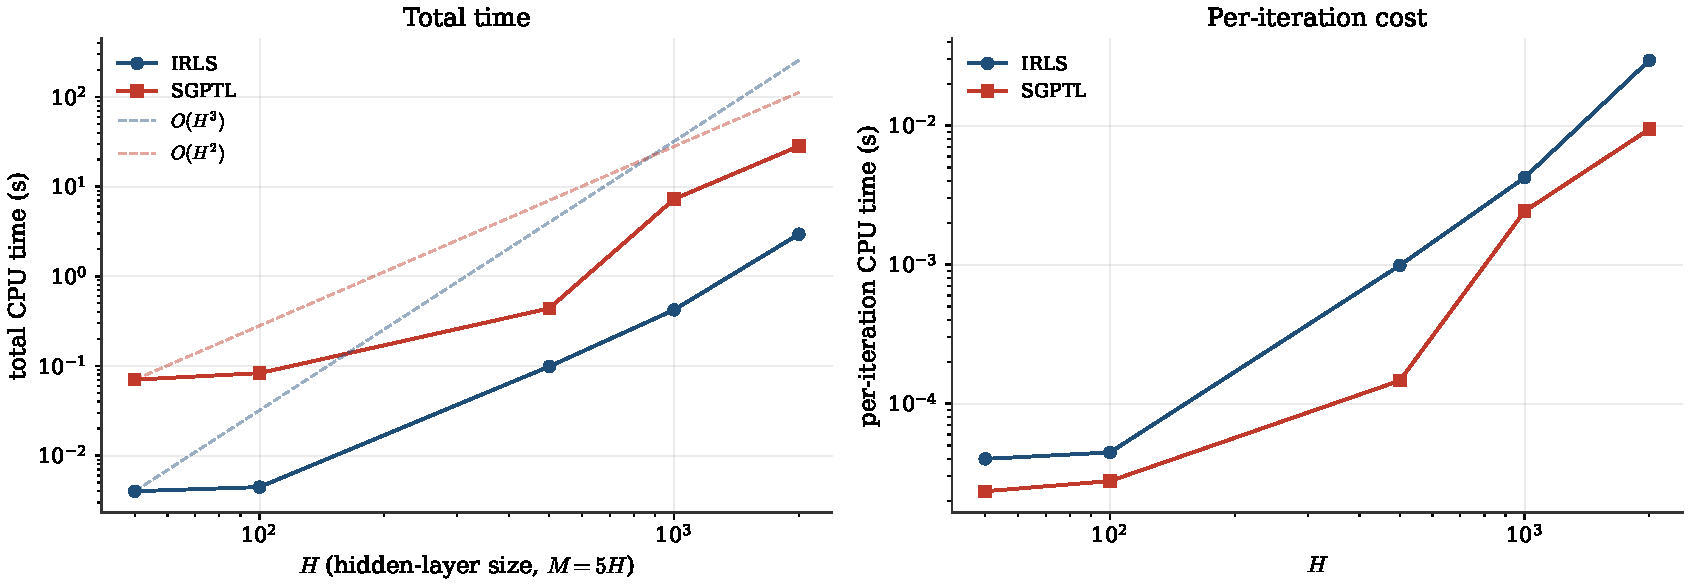
\includegraphics[width=\textwidth]{images/scalability.pdf}
    \caption{Scaling of wall-clock time with $H$ at $M=5H$. Left:
    total time on log-log axes; the dashed blue line is the
    $O(H^{3})$ reference. Right: per-iteration cost.}
    \label{fig:scalability}
\end{figure}

The crossover predicted in Section~\ref{sec:comp_cost}
($H^{3}\gtrsim MH$, i.e. $H^{2}\gtrsim M$) does not occur in this
regime, because $M=5H$ keeps $M\sim H$ while the crossover requires
$M\ll H^{2}$. We should expect to see the regime shift only when $M$
is much smaller than $H^{2}$, i.e. when there are very few training
samples relative to the hidden-layer size. On the project's intended
ELM regime ($M\gg H$) IRLS dominates not just in iterations-to-target
but also in raw wall-clock time.

\section{Iterations to a target accuracy}
\label{sec:iters-to-eps}

A different way to read the same data is to ask how much work each
algorithm needs to reach a fixed accuracy~$\varepsilon$ on the same
instance. Table~\ref{tab:iters-to-eps} reports iteration counts and
wall-clock times to the first iterate satisfying $f-f^{*}\le
\varepsilon$ on the moderate problem ($H=50$, $M=200$,
$\lambda_\text{LASSO}=0.1$).

\begin{table}[H]
    \centering
    \begin{tabular}{rrrrr}
        \toprule
        $\varepsilon$ & $k_\text{IRLS}$ & $t_\text{IRLS}$ (s) &
        $i_\text{SGPTL}$ & $t_\text{SGPTL}$ (s) \\
        \midrule
        $10^{-1}$ & $  1$ & $4.4\cdot 10^{-5}$ & $    3$ & $7.4\cdot 10^{-5}$ \\
        $10^{-2}$ & $  3$ & $1.2\cdot 10^{-4}$ & N/A & N/A \\
        $10^{-3}$ & $  7$ & $2.2\cdot 10^{-4}$ & N/A & N/A \\
        $10^{-4}$ & $ 19$ & $5.4\cdot 10^{-4}$ & N/A & N/A \\
        $10^{-6}$ & $101$ & $2.6\cdot 10^{-3}$ & N/A & N/A \\
        \bottomrule
    \end{tabular}
    \caption{Iterations and wall-clock time required to reach
    $f-f^{*}\le\varepsilon$ on the moderate problem ($H=50$,
    $M=200$, $\lambda_\text{LASSO}=0.1$). N/A means the gap was not
    reached within the $30000$-iteration SGPTL budget.}
    \label{tab:iters-to-eps}
\end{table}

The two algorithms are competitive only at the loosest accuracy:
SGPTL reaches $\varepsilon=10^{-1}$ in three iterations, IRLS in one,
and at this scale the per-iteration cost difference dominates so the
two times are within a factor of two of each other. Past $10^{-1}$ the
SGPTL trajectory plateaus and the algorithm fails to reach $10^{-2}$
within the $30000$-iteration budget on this instance. IRLS adds a small
near-constant number of iterations per decade
($1\to 3\to 7\to 19\to 101$, between $2.7\times$ and $5.3\times$ per
decade) and reaches $10^{-6}$ in $101$~iterations. The contrast is the
practical illustration of what Section~\ref{sec:comp_summary} predicted
from the $O(\log\varepsilon^{-1})$ versus $O(\varepsilon^{-2})$
comparison: at $\varepsilon=10^{-2}$ the worst-case
$\Omega(L^{2}/\varepsilon^{2})$ lower bound for SGPTL on this instance
size already exceeds the $30000$-iteration budget once the constants
are taken into account.

Figure~\ref{fig:comparison} overlays the two trajectories on the same
instance.

\begin{figure}[H]
    \centering
    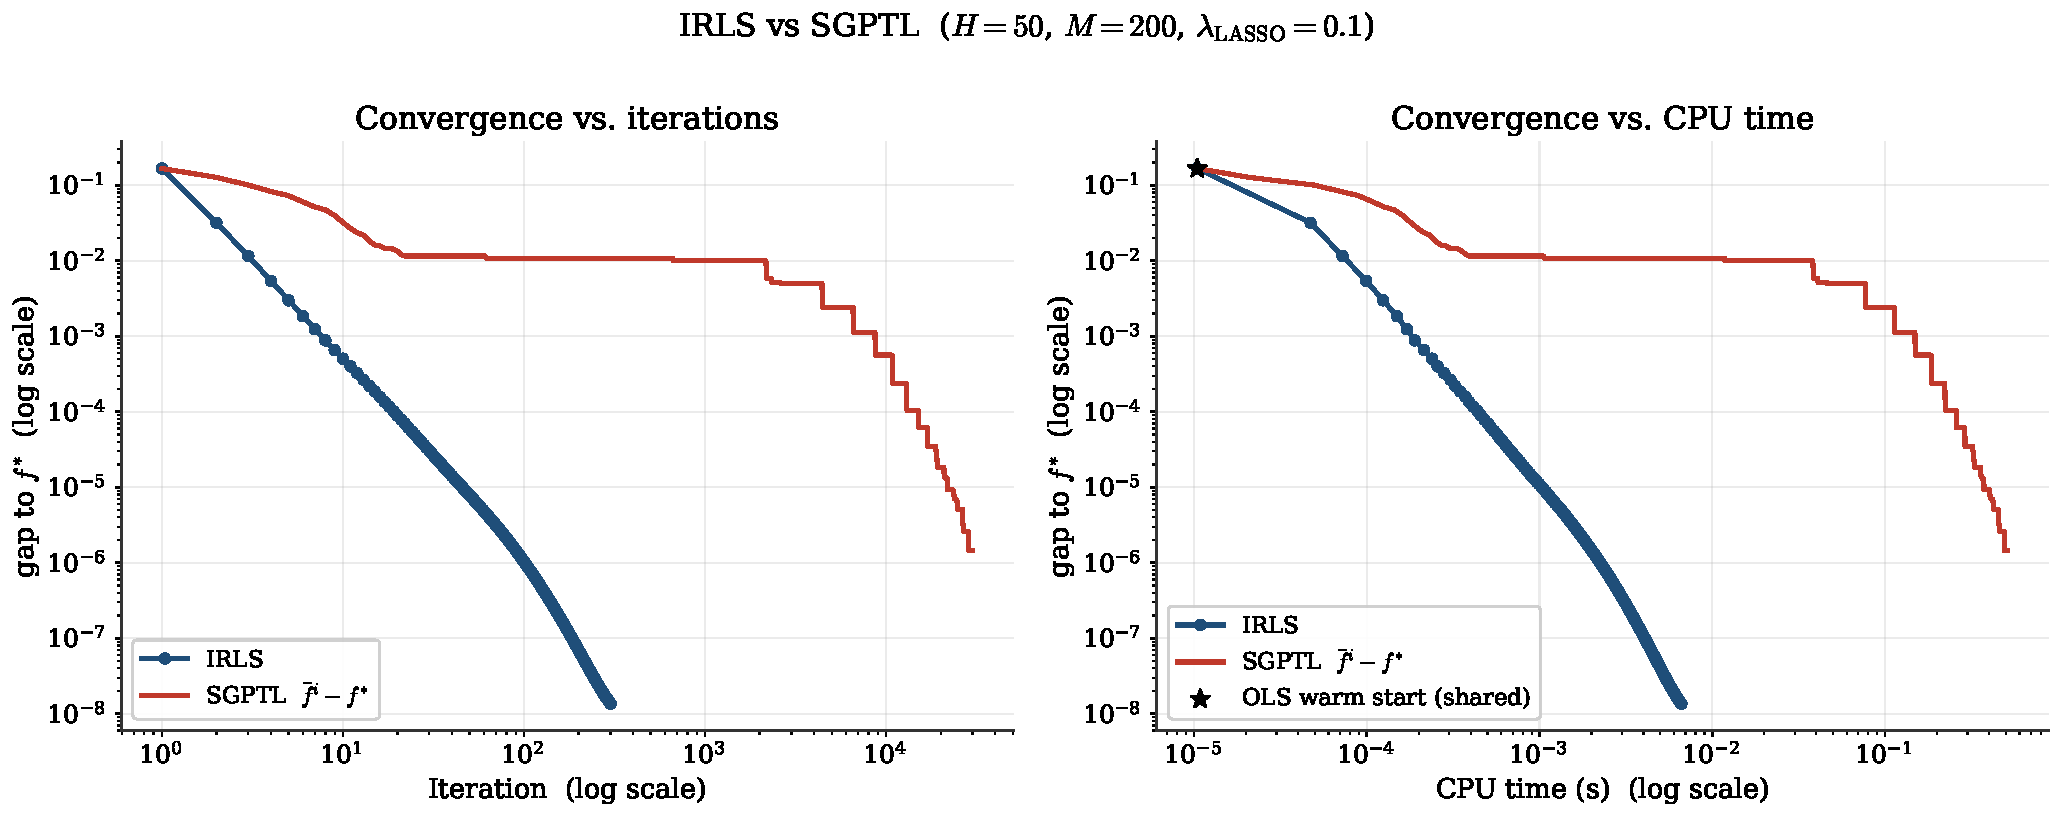
\includegraphics[width=\textwidth]{images/comparison_irls_dsm.pdf}
    \caption{IRLS versus SGPTL on the moderate problem. Left:
    optimality gap versus iteration. Right: gap versus CPU time.}
    \label{fig:comparison}
\end{figure}
